\documentclass[12pt]{report}
\usepackage[a4paper, portrait, margin=0.75in]{geometry}
\usepackage{graphicx} % Required for inserting images
\usepackage[page,toc,titletoc,title]{appendix}
\usepackage{mathptmx}
\usepackage{pdflscape}
\usepackage{pdfpages}
\usepackage{enumitem}
\usepackage{hyperref}
\usepackage{cleveref}

\title{Integrating streamed sensor data into a distributed model of a complex system \\
\large{A report submitted in partial fulfilment of the requirements for the degree of \\
\textbf{Bachelor of Engineering (Hons) in Software Engineering} \\
at \\
\textbf{the University of Waikato}
}}

\author{Bert Downs  \\ 
Supervised by Tim Walmsley, Mark Apperley }

\date{October 2024}

\begin{document}

\maketitle


\chapter*{Abstract}

Modern factories are equipped with a variety of sensors that monitor the state of the factory and products. To fully utilise this sensor data, the field of Digital Twinning is emerging, which combines live factory data, historical state, and a model of the factory to predict future states. The process of creating a digital twin lacks standardization. This project presents a standardised framework for creating digital twins of chemical plants, using the Ahuora Digital Twin Platform and industry standard data processing tools. The framework is evaluated in a case study of a heat pump dryer, demonstrating the potential of digital twins to improve factory performance.

% TODO: Something about results and evaluation stuff.
% this report argues that

\chapter*{Acknowledgements}

I would like to thank my supervisors, Tim Walmsley and Mark Apperley, for their guidance and support throughout this project. I would also like to thank the Ahuora project team for their assistance and feedback. Finally, I would like to thank my family and friends for their encouragement and support.

\tableofcontents

\listoffigures

\listoftables

\newpage

\chapter{Preface: The Ahuora Digital Twin Platform}


%This chapter has been included based on feedback from the mid-progress report that the marker did not understand the context of the project.
\textit{ Unlike many other projects, this project is part of a larger, multi-disciplinary project. Occasionally, work has focused on broader platform development rather than solely on this sub-project. Additionally, some work involves research for future implementations that cannot be completed with the platform's current capabilities. This chapter provides an overview of the Ahuora Digital Twin Platform, to provide context for the rest of the report.}

\section{Background}

`Project Ahuora' is a Ministry of Business, Innovation and Employment (MBIE) funded project that aims to decarbonise the process heat sector. 
By decarbonising, New Zealands' greenhouse gas emissions will be reduced. Cost savings from reduced energy consumption are anticipated, along with increased energy independence.
This is a multi-disciplinary project that involves researchers from the University of Waikato, University of Auckland, Massey University,
and other global universities. Chemical Engineers bring understanding of the chemical processes that are used in industry. Electrical Engineers bring understanding of the grid system
and how to integrate renewable energy sources. Mechanical engineers bring understanding of how to design and build more efficient systems. Software Engineers bring understanding of how to
model, simulate, and monitor complex systems. 

A key objective is to develop a digital twin platform for the chemical processing industry. This platform will allow New Zealand factory operators to model their processes, simulate different scenarios, and monitor their processes in real-time.
This will enable factory operators to make data-driven and scientifically backed decisions on how to improve their processes. A digital twin can recognise where the factory is underperforming, suggest real-time improvements, and help plain future investments.  

\section{The Ahuora Simulation Platform}

A key deliverable of the Ahuora project to date is the Ahuora Simulation Platform. This is a web-based platform that allows users to model a factory or other energy system, and simulate its performance. The platform is based on the IDAES Process Systems Engineering Framework, which is a Python library that provides tools for modelling and simulating chemical processes. 

Currently, the platform can model a factory at a single point in time. The user specifies the properties of the factory, such as the flow rates of different materials, the temperature and pressure of different streams, and the efficiency of different unit operations. The platform then simulates the factory and provides the user with a report on the factory's performance.

\subsection{Flowsheet Interface}


\begin{figure}
    \centering
    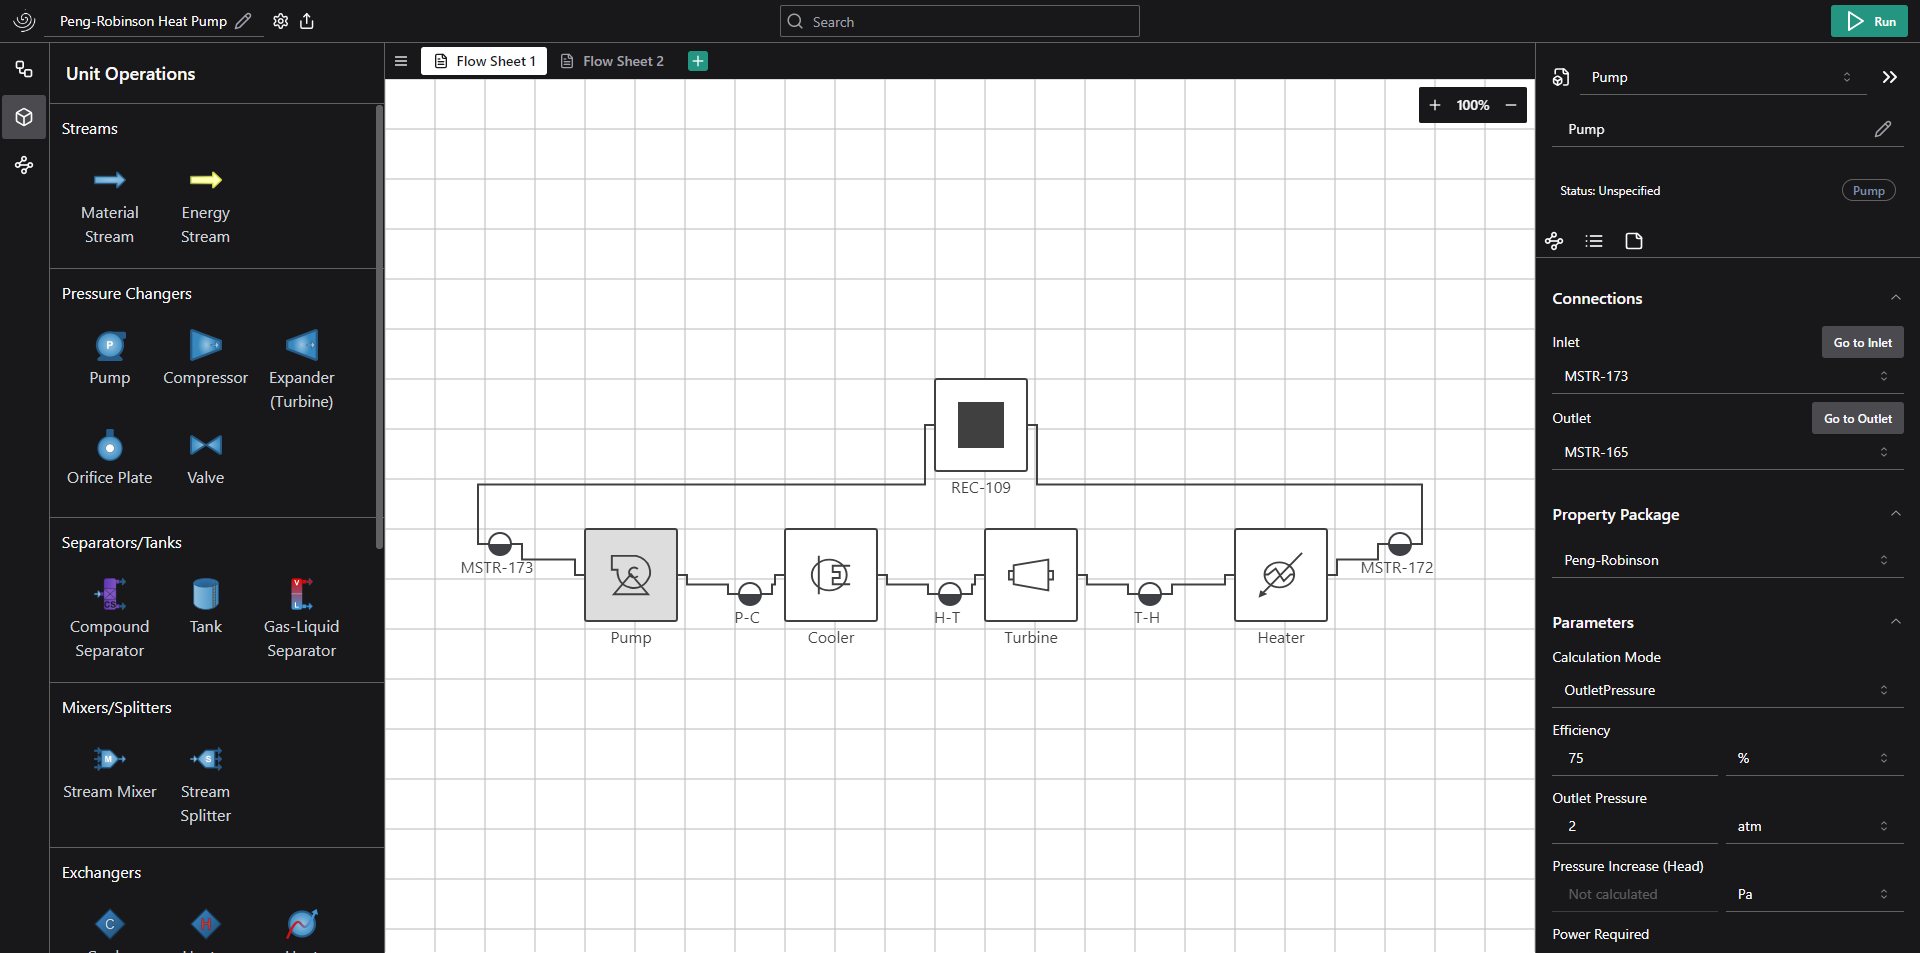
\includegraphics[width=\textwidth]{platform_screenshot.png}
    \caption{Example Flowsheet in the Ahuora Simulation Platform}
    \label{fig:platform}
\end{figure}

\Cref{fig:platform} shows a screenshot of the Ahuora Simulation Platform, as at August 2024. The user interface is divided into three main sections. The left-hand panel shows a list of unit operations from a factory, including pumps, heaters, heat exchangers, reactors, and material streams. The user can drag and drop these unit operations onto the canvas in the centre of the screen. The user can then connect the unit operations together to create a process flow diagram. The right-hand panel shows the properties of the selected unit operation, such as the flow rate of the material stream, the temperature and pressure of the stream, and the efficiency of the unit operation. The user can edit these properties to simulate different scenarios.

The displayed flowsheet shows a simple heat pump cycle. The block on the top is a ``recycle", specifying that the output of the cooler is fed back into the pump. A more complex flowsheet would replace the cooler and heater with heat exchangers, which exchange heat with their environment, but this provides a simple example.

\subsection{Online Integration}

\begin{figure}
    \centering
    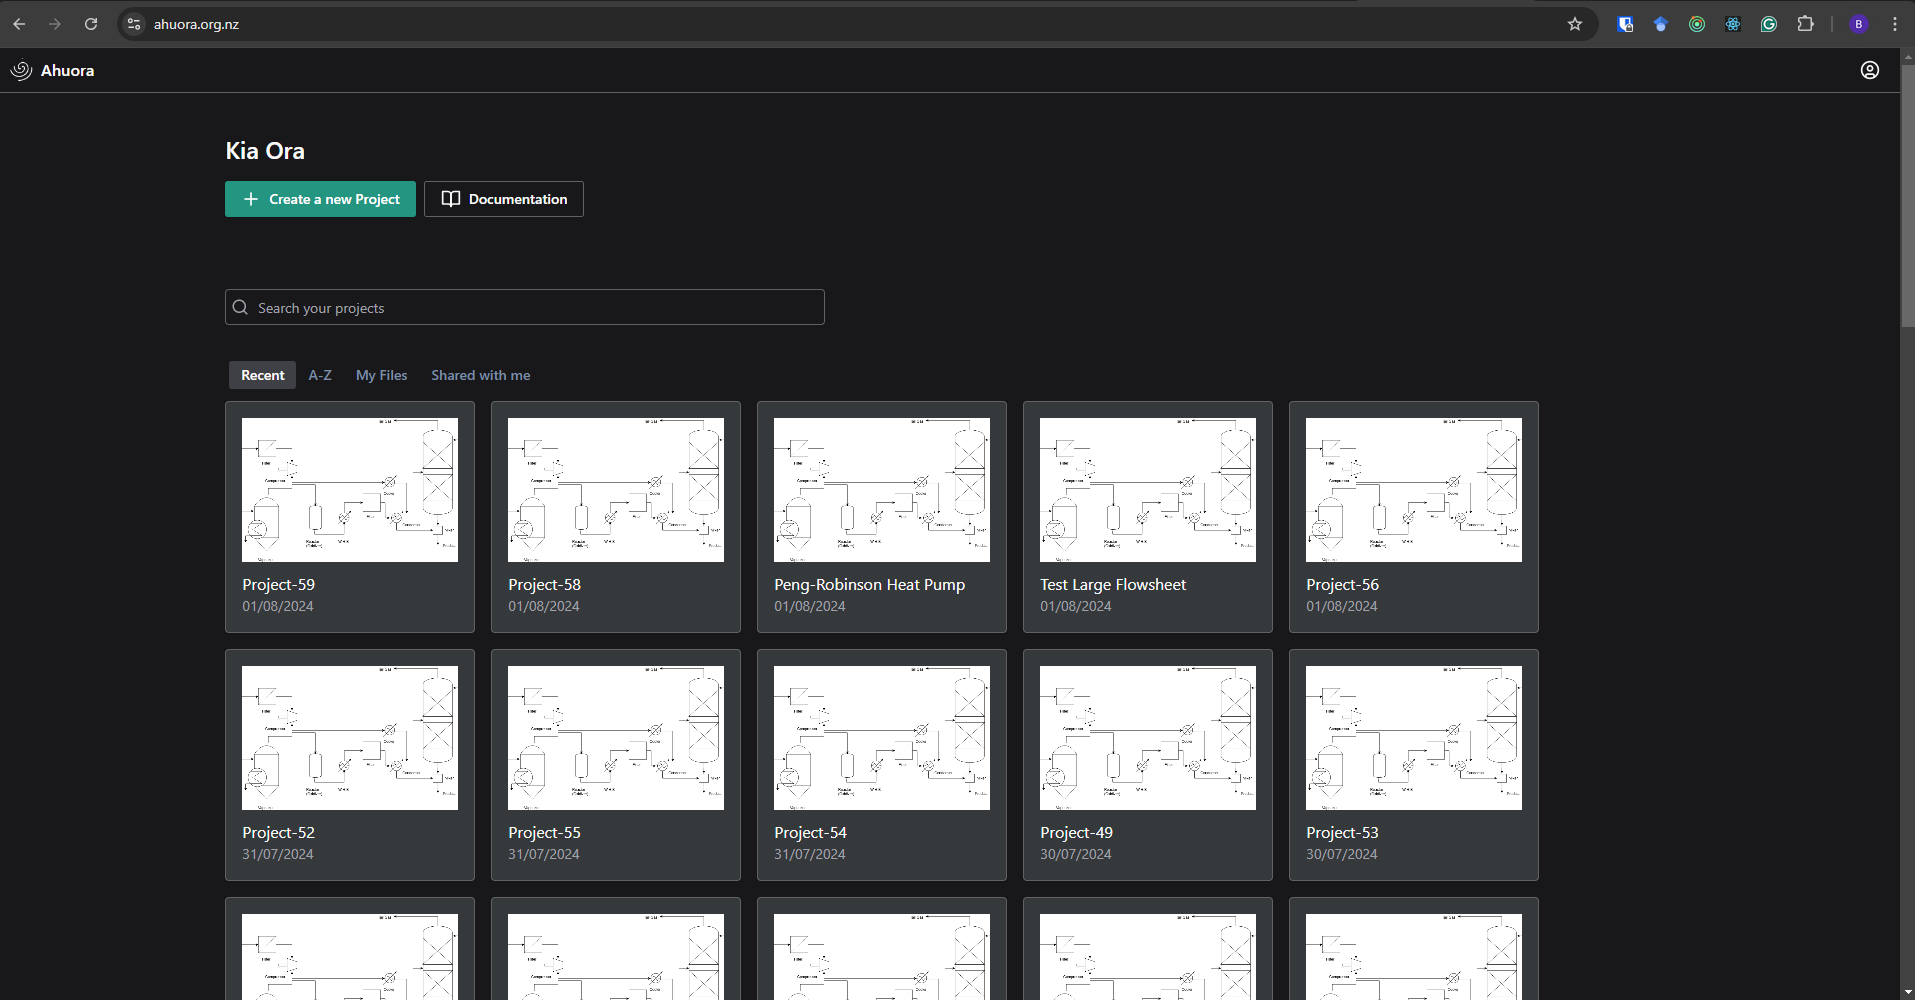
\includegraphics[width=\textwidth]{platform_homepage.png}
    \caption{Homepage of The Ahuora Simulation Platform}
    \label{fig:homepage}
\end{figure}

The Ahuora Simulation Platform is designed as a web-based multi-user platform. This offloads processing and data storage to the server, allowing users to access the platform from any device with a web browser. Simulation can be very computationally expensive, particuarly in advanced models, so this is a key feature. It enables simulation to be run in parallel on powerful servers, and allows the platform to be used in industry without requiring significant upfront investment in hardware. In future, this will also enable the platform to be used for real-time collaboration between multiple users. Its API allows it to be integrated with other software, enabling enhanced functionality, real-time updates, and broader interactions.

The home page of the platform, shown in \cref{fig:homepage}, provides a list of saved simulations, and allows the user to create a new simulation. This is not publicly acessible, as the platform is still in development, and user account functionality is not yet complete.

\section{The Ahuora Digital Twin Platform}

There are a number of objectives that Ahuora is working towards including in the platform. These include:

\begin{itemize}
    \item Steady-state Process Simulation: This is the current state of the platform. However, it can be improved by adding support for:
    \begin{itemize}
        \item More unit operations, defined from first principles equations
        \item Custom unit operations
        \item Unit operations defined from data (Machine Learning \& Hybrid Modelling)
        \item More property packages (enabling accurate simulation of a wider range of chemical processes)
        \item Support for more advanced mathematical constraints
    \end{itemize}
    \item Advanced analysis techniques: This includes:
    \begin{itemize}
        \item P-Graph Analysis, generating and comparing alternative process structures
        \item Pinch Analysis, to identify the theorical minimum energy consumption of a process
        \item Heat Exchanger Network analysis, to identify opportunities for heat recovery in individual processes
        \item Utility System Analysis, to identify opportunities for energy savings on a plant-wide scale
    \end{itemize}
    \item Process Variable Optimisation: Calculating the optimal operating conditions (temperatures, pressures, flow rates, power utilisation) for a given process
    \item Dynamic simulation, to model the factory over time, so that the effect of changes on can be predicted
    \item Process Scheduling, to optimise the factory's resources across tasks
    \item Live Data Processing, to:
    \begin{itemize}
        \item simulate plant conditions in real-time, for performance monitoring and diagnostics
        \item update the simulation based on real-world changes, e.g fouling or equipment degradation
    \end{itemize}
    \item Process Control - adjusting the physical process plant based on the simulation to maintain desired operating conditions
    \item Reporting functionality, such as Process \& Instrumentation diagrams.
\end{itemize}

For clarity in this report, the term ``Ahuora Digital Twin Platform" will refer to the complete solution, keeping in mind all these future objectives. The term ``Ahuora Simulation Platform" will refer to the current state of the platform, which is based on steady-state simulation, and does not yet support the features required for a Digital Twin.

\section{The Role of This Project}

This project contributes to a number of these objectives, utilising the Ahuora Simulation Platform as a base, updating it to work with real-time data, and developing a standardised framework for integrating real-time sensor data into the platform. This provides the groundwork to support the advanced analysis techniques, process variable optimisation, dynamic simulation, and live data processing that are required for a Digital Twin.

\chapter{Introduction}

% Some sort of hook, surely someone somewhere said "data is the new gold" or something

% State the argument you will make in the report

\section{Motivation}

Ahuora is a research group focused on developing smart energy systems to decarbonise factories. They have developed a Web-based simulation platform that allows users to create a digital twin of their factory. 
This platform is based on steady-state simulation, which simulates a factory at a single point in time. All factory conditions are manually specified by the user.
This platform is useful for modelling changes to a factory before construction, or understanding the factory's performance under different conditions.

However, their platform cannot be considered a ``Digital Twin'' because it does not take into account the factory's real-time state.
By integrating real-time sensor data into the simulation, the platform can monitor the factories' performance, and suggest tunings that will optimise resource efficiency.
The data can also be used to predict and avoid failures and downtime, a key problem where many resources are wasted.
Additionally, models created in the Ahuora Simulation Platform during the design phase could also be used during operation, minimising overhead costs.

Including real-time data in the simulation is needed to improve the usefulness of the Ahuora Platform in industry. 
The system needs to meet industry requirements for security, scalability, and reliability. As such, this project 
has been commissioned to develop a standardised framework to enable the integration of real-time sensor data into the Ahuora Digital Twin Platform.

% Todo: Include a substantial section explaining the Ahuora Digital Twin Platform, and what it does. THis is a necessary background for the project. The marker won't understand otherwise.

\section{Objectives}

The objectives of this project are as follows:
\begin{itemize}
    \item Conduct a literature review on Digital Twins, Digital Twin Platforms, and Data Processing Tools.
    \item Conduct an Exploratory Analysis of techniques and tools for digital twin development, based on their applicability to the Ahuora Digital Twin Platform and the requirements of live data processing.
    \item Develop the Ahuora Digital Twin platform to a stage where support for live data processing can be added.
    \item Develop a standardised framework for integrating real-time sensor data into the Ahuora Digital Twin Platform.
    \item Develop a prototype implementation of the framework.
    \item Evaluate the prototype implementation in a case study.
    \item Identify areas for future work.
\end{itemize}
\section{Scope}

Full integration of real-time sensor data into the Ahuora Digital Twin Platform is out of scope for this project. 
This project will focus on identifying techniques and tools for simulation and modelling that will be needed in a industry setting,
and developing a prototype live data processing system for Ahuora that is extensible enough to support those techniques and tools.


\section{Literature Review}


\subsection{Digital Twins}

\subsection{Digital Twin Platforms}

\subsection{Data Processing Tools}


\chapter{Methodology}
% helicopter view, structure of the report

Because of the scope of the 

This project was conducted in three main stages: Research, Development, and Evaluation. 

\section{Research}

The research stage involved small-scale experiments in the IDAES framework to test the feasibility of integrating live data processing techniques into the Ahuora Digital Twin Platform. This followed directly from the Literature Review, which identified a variety of modelling techniques that could be used in a Digital Twin Platform. The research stage was used to identify the requirements for the Ahuora Digital Twin Platform, and to develop a high-level architecture for the platform that would support these requirements.

\section{Development}

The development stage involved developing a pilot implementation of the framework. This was done seperate from but in conjunction with the Ahuora Simulation Platform, following the architecture developed in the research stage. While the research stage focused on choosing an architecture that would support future requirements, the development stage focused on implementing a pipeline that worked with the current capabilities of the Ahuora Simulation Platform. 

\section{Evaluation}

The evaluation stage involved testing the pilot implementation in a case study. This was done by developing a model of a heat pump dryer in the Ahuora Simulation Platform, and integrating real-time sensor data into the model. The case study was used to evaluate the feasibility of the framework, and to identify areas for future work.

\chapter{Architecture Research}

This project was conducted as part of a real-world, collaborative effort to build the Ahuora Digital Twin platform, so the methodology followed engineering principles, rather than being purely academic experimentation. Research into live data processing techniques could only be conducted as far as the Digital Twin Platform supported them. The focus of the project moved between improving the Simulation Platform to support more modelling techniques, and developing a live data processing system that could be integrated into the platform.

\section{Experimentation in IDAES}

The Ahuora Digital Twin Platform is built on top of the IDAES Process Systems Engineering Framework. Because of this, the IDAES framework was used as a testbed for experimentation with live data processing techniques. The IDAES framework is a Python library that provides tools for modelling and simulating chemical processes. It is designed to be extensible, so that new modelling techniques can be added to it. 


From the Literature Review, a variety of modelling techniques were identified, including Dynamic Modelling, Surrogate Modelling, and Optimisation. The Ahuora Digital Twin platform is currently based on steady-state simulation and does not support these techniques. The IDAES framework was used to test the feasibility of integrating live data processing techniques into the Ahuora Digital Twin Platform. This will enable the live data platform to be designed in a way that supports these techniques being added in the future.


\subsection{Dynamic Modelling}

I used the IDAES framework to develop a dynamic model of a steam tank, with a valve controlling the inlet and outlet pressure and flow rate. A PID controller was used to control the valve opening fraction to regulate the pressure in the tank.

\begin{figure}
    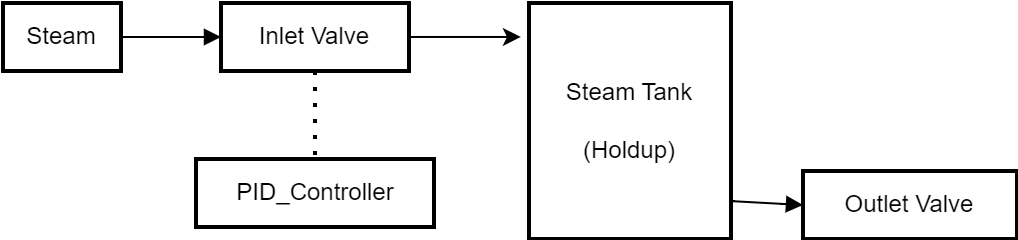
\includegraphics[width=0.9\textwidth]{dynamicmodelling.png}
    \caption{Dynamic Modelling of a Steam Tank}
    \label{fig:dynamicmodelling}
\end{figure}

This provided a simple example of a dynamic system. The inlet and outlet valve and the PID controller were not dynamic models: From a mathematical perspective, this means their properties were fully determined by the inlet and outlet conditions. The only dynamic model was the Steam Tank. From a mathematical perspective, this means that the state of the steam tank was determined by the inlet and outlet conditions, but also the previous state of the tank, i.e how ``full" the tank is.


\subsubsection{Key Findings}

\begin{itemize}
    \item The IDAES framework is well-suited to dynamic modelling, as it provides tools for creating and solving differential equations. It can easily model the same system at different time scales.
    \item The Ahuora Simulation Platform will require substantial changes to support dynamic modelling. Rather than storing a single value for each property, it will need to store the state of each property at each time step.
    \item This will also require significant UI changes to view the state of the system at different time steps. This could be achieved through some sort of time slider, and graph visualisations of properties over time.
    \item Specifying the initial conditions of the system will be more complex, as the user will need to specify the initial state of dynamic properties, such as the initial tank level. Other properties, such as the valve opening fraction, will need to be specified as functions of time.
\end{itemize}

\subsection{Surrogate Modelling}

Surrogate Modelling is the process of creating a simplified model of a complex system. This is usually done using machine learning techniques. This provides a good test case of implementing data-driven modelling techniques in the IDAES framework.

IDAES includes a framework for data-driven modelling called PySMO. This provides utilities for training polynomial, Radial Basis Function, and Kriging models to approximate the behaviour. 

\subsubsection{Key Findings}

Surrogate Modelling may be achieved using IDAES's built-in PySMO libraries, or other similar libraries such as OMLT. It is reasonably straightforward to train a surrogate model to represent a non-dynamic unit operation, but dynamic unit operations get significantly more complex - instead of modelling a single value, the surrogate model must be able to model the entire time system. There are some methods of doing this, such as using neural ODEs, Residual Networks, Operator Networks, or some other sort of convolutional network. There is little research into applying these methods in the field of chemical and process simulation, especially in the context of mathematical modelling such as the IDAES framework.

The exact same process for surrogate modelling can also be used to model unit operations from historical data. This is useful when there is no mathematical model of the unit operation, but there is historical data available. This would be very useful when applying the Ahuora Digital Twin Platform to existing factories, where the exact mathematical properties of the unit operations are unknown but there is a wealth of historical data available. Online Learning techniques could be used to update the surrogate model in real-time, as new data becomes available. This is a key step in turning a ``simulation" into a ``digital twin", as it allows the model actively adapt to real-world conditions.

Because of the limited functionality of the Ahuora Digital Twin Platform, it is currently beyond the scope of this project to implement a surrogate model. However, the IDAES framework is well-suited to this task, and it is likely that a surrogate model could be implemented in the future.

Additionally, the Ahuora Digital Twin Platform will need a user interface to support creating these different types of models. As surrogate modelling is a complex process, the user interface will need to be able to guide the user through the process of creating a surrogate model from a dataset, and provide feedback on the quality of the model. This will require a significant amount of work, and will likely be a key focus of future development. 


\subsection{Optimisation and Control}


\subsubsection{Key Findings}

Implementing Model Predictive Control in IDAES is relatively straightforward, as long as there is a dynamic model of the system, a cost function, and the optimisation problem is well-posed. The Ahuora Digital Twin Platform does not support optimisation yet, but this will be supported in the future. 

IDAES's Caprese library can simulate model predictive control, but in order for it to truly be useful IDAES needs to be paired with a real-time data processing system. The real-time data processing system will need to be able to make the controlling actions suggested by the MPC in real-time, and then inform the MPC of the system's response. This requires integration with the industry-specific SCADA systems that are used to control factories.

This project will focus on the data-gathering and processing aspects of this problem, rather than the control aspects. As time permits, suggestions will be made on how the control aspects could be implemented.



The research in the literature review and the experimentation in IDAES provided a good understanding of the requirements for the Ahuora Digital Twin Platform. The next step was to develop a architecture for the platform that would support these requirements. A pilot implementation was then developed to demonstrate the feasibility of the architecture.

\subsection{Architecture}

The current Ahuora Simulation Platform is split into three main parts:

\begin{itemize}
    \item The Frontend UI, which is written in Typescript/React and runs in the user's web browser. This is responsible for rendering the flowsheet, and allowing the user to interact with the simulation.
    \item The Backend API, which is written in Python/Django and runs on the server. This is responsible for storing the simulation data, orchestrating calls to run the simulation, and returning the results to the user.
    \item The IDAES solving engine, which is written in Python and runs on the server. This is responsible for solving the simulation, and returning the results to the API. It has been seperated out from the API to allow it to be scaled independently.
\end{itemize}


\begin{figure}
    \centering
    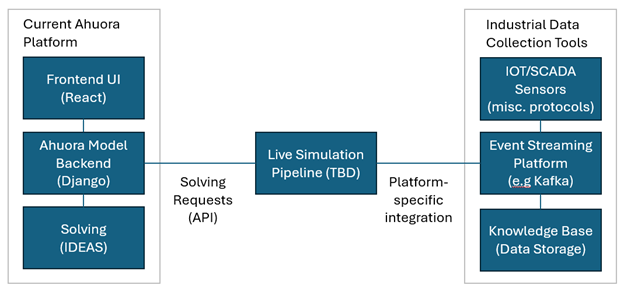
\includegraphics[width=0.9\textwidth]{architecture.png}
    \caption{Anticipated method of implementing the Ahuora Simulation Platform into an industrial system.}
    \label{fig:architecture}
\end{figure}

% TODO: Explain industrial data collection tools, how our stuff fits in.
Additionally, there are also a number of other tools that are used in industry for collecting and processing sensor data. There may be an integrated solution or a number of different tools that are used together, but they can be grouped by their functionality:
\begin{itemize}
    \item Data Collection: These tools are responsible for collecting data from sensors and storing it in a database. They may also provide tools for cleaning and preprocessing the data. This includes IoT networks and SCADA systems.
    \item Data Processing: These tools are responsible for processing the data to extract useful information. This may include machine learning models, statistical analysis, or other data processing techniques. Generally, these tools will sit within some sort of framework or pipeline, such as Apache Kafka, Flink, or a custom solution.
    \item Data Storage: These tools are responsible for storing the data in a way that is accessible to the other tools. This may include databases, data lakes, or other storage solutions. In Model-Based Systems Engineering, this is often referred to as a Knowledge Base.
\end{itemize}





% Impact, or conclusions, or something
\section{Impact} 



\chapter{Development}


\section{Minimum Viable Product}

\section{Extensions}



\chapter{Functional Example: Heat Pump Dryer}

\section{Motivation}

\section{Method}

\section{Results}

\section{Discussion}

% Strengths, limitations, impacts, what could have been better, etc


% evaluates the broader impact of the project outcome, either quantitatively or qualitatively (e.g., social, economic, environmental, health, safety, legal, ethical, and/or cultural issues)
\section{Impact}

\chapter{Conclusions}

% Present the outcome, and the arguments

\section{Future Work}

\chapter{References}

\bibliographystyle{unsrt} % We choose the ``plain" reference style
\bibliography{refs} % Entries are in the refs.bib file

\begin{appendices}



% \chapter{Project Proposal} \label{sec:proposal}
% The project proposal is included as an appendix on the following page.


% 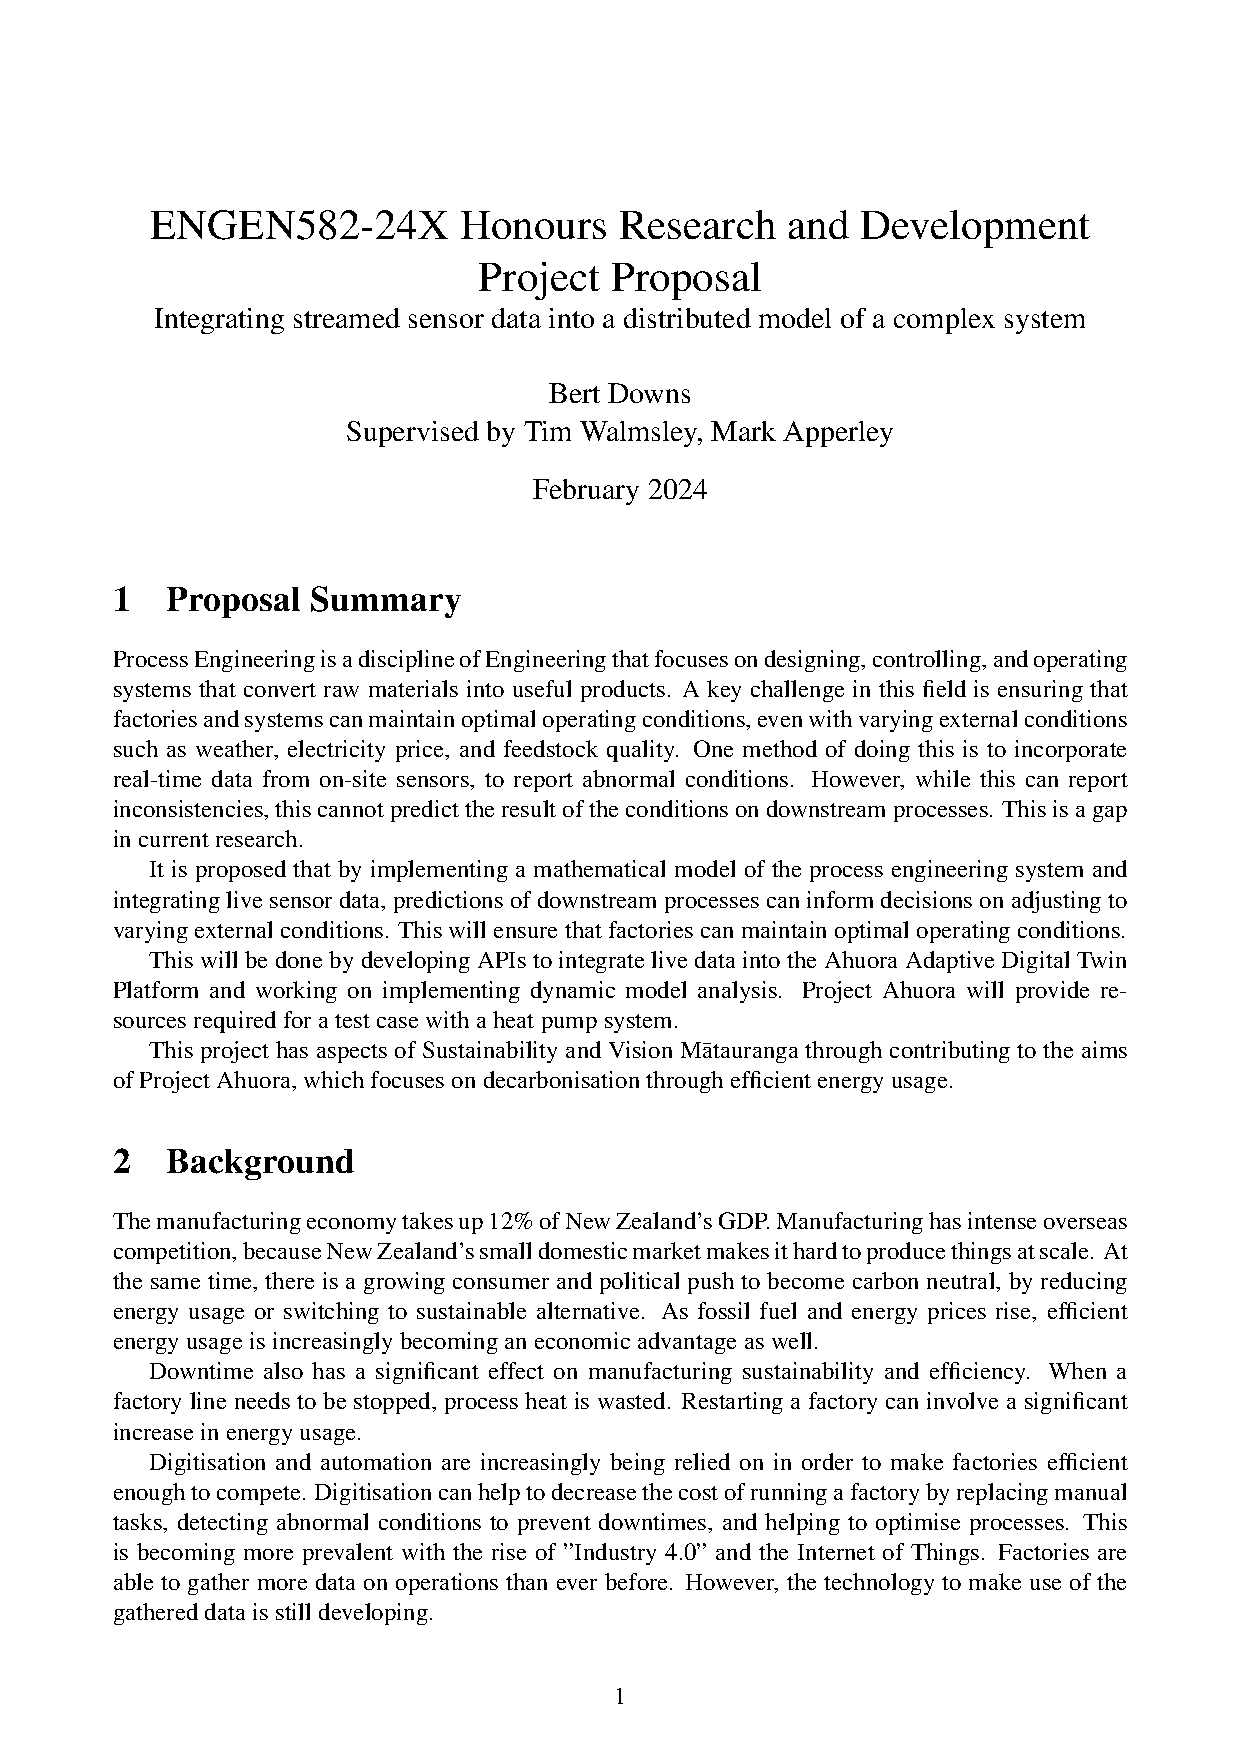
\includepdf[pages=1-4]{proposal.pdf}

% \begin{landscape}
%     \includepdf[pages=5,angle=90]{proposal.pdf}
% \end{landscape}

% \chapter{Literature Review} \label{sec:litreview}
% The literature review is included as an appendix on the following page.

% 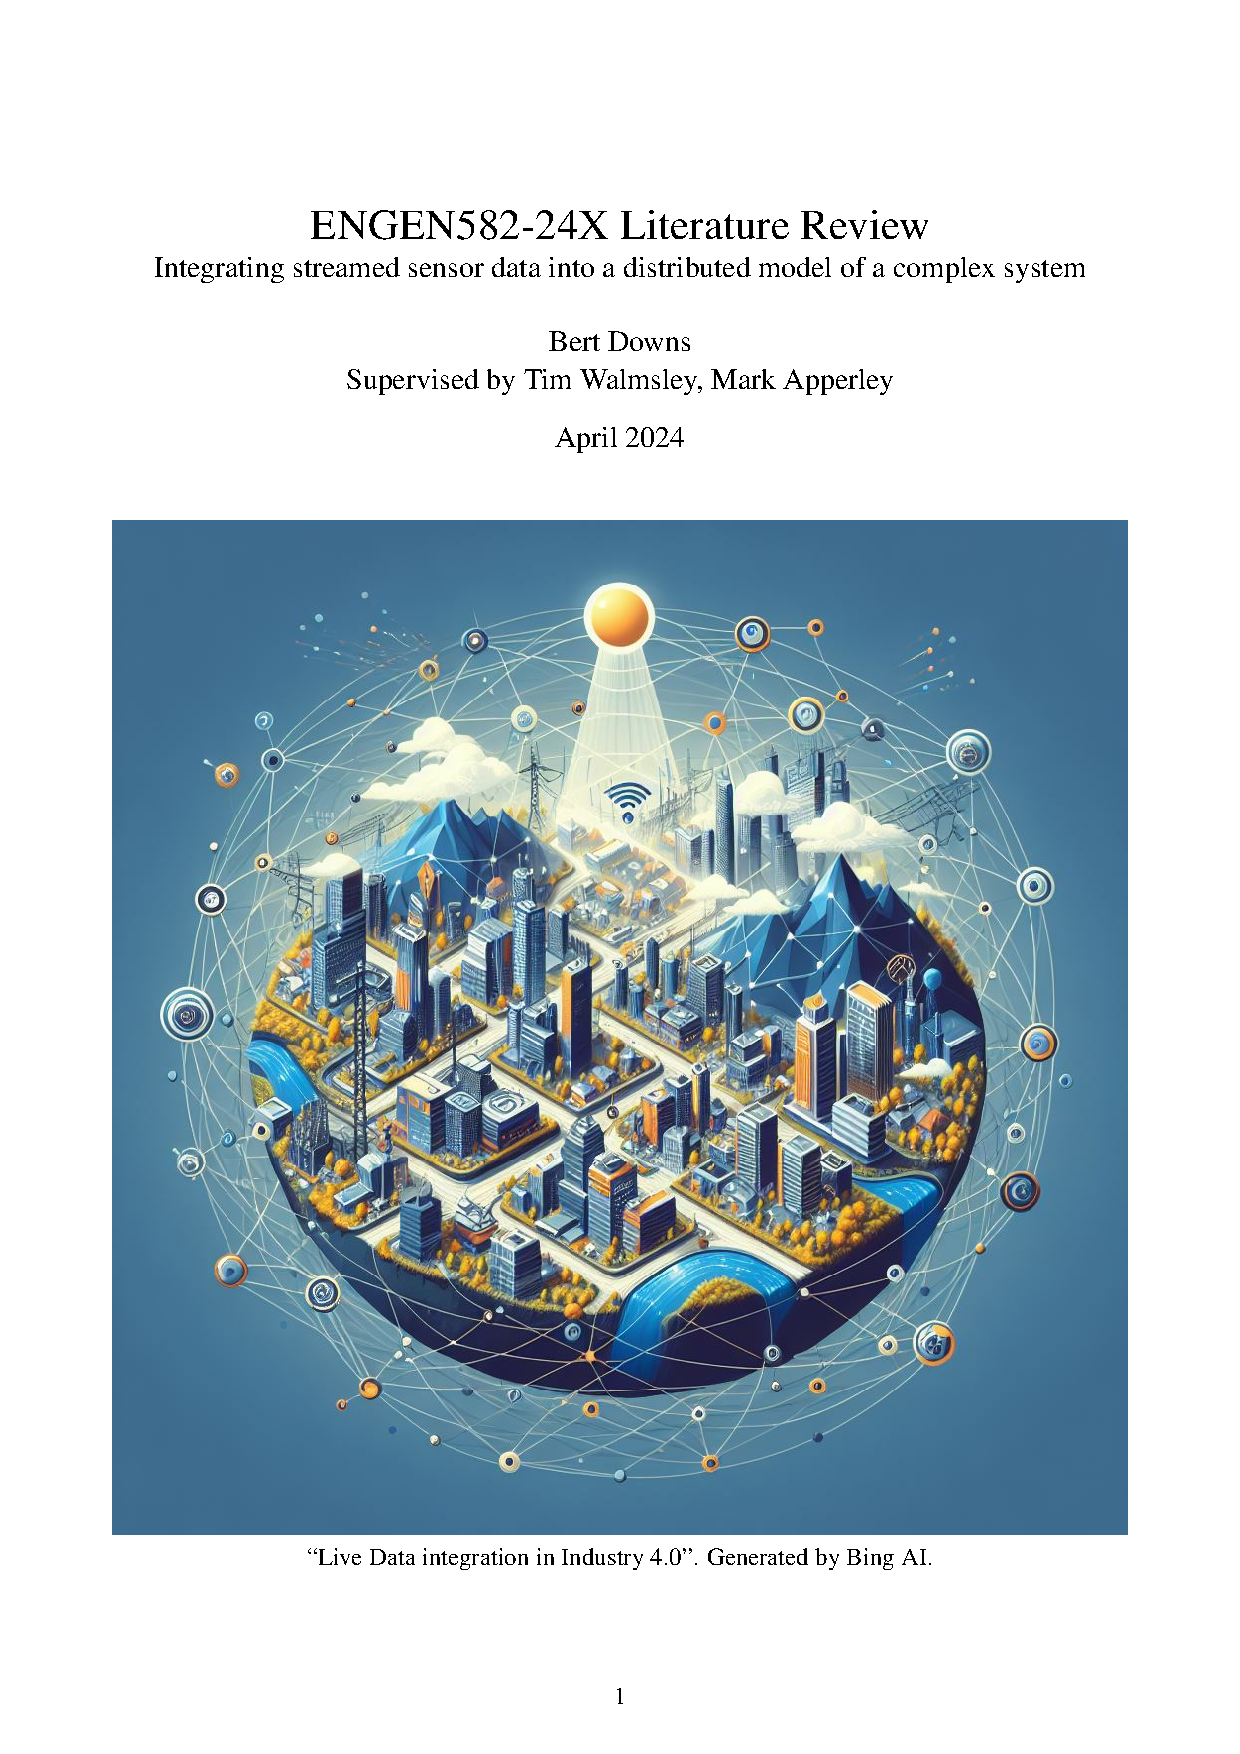
\includepdf[pages=-]{literature_review.pdf}

\end{appendices}
\end{document}